\documentclass{beamer}
\usepackage[utf8]{inputenc}
\usepackage{graphicx, epsfig}
\usepackage{amsmath,mathrsfs,amsfonts,amssymb}
%\usepackage{subfig}
\usepackage{floatflt}
\usepackage{epic,ecltree}
\usepackage{mathtext}
\usepackage{fancybox}
\usepackage{fancyhdr}
\usepackage{multirow}
\usepackage{enumerate}
\usepackage{epstopdf}
\usepackage{multicol}
\usepackage{algorithm}
\usepackage[noend]{algorithmic}
\usepackage{tikz}
\usepackage{blindtext}
\usetheme{default}%{Singapore}%{Warsaw}%{Warsaw}%{Darmstadt}
\usecolortheme{default}
\setbeamerfont{title}{size=\Huge}
\setbeamertemplate{footline}[page number]{}


\makeatletter
\newcommand\HUGE{\@setfontsize\Huge{35}{40}}
\makeatother    

\setbeamerfont{title}{size=\HUGE}
\beamertemplatenavigationsymbolsempty

% latin bold lower
\newcommand{\ba}{\mathbf{a}} 
\newcommand{\bc}{\mathbf{c}} 
\newcommand{\be}{\mathbf{e}} 
\newcommand{\bh}{\mathbf{h}} 
\newcommand{\bp}{\mathbf{p}} 
\newcommand{\bt}{\mathbf{t}} 
\newcommand{\bs}{\mathbf{s}} 
\newcommand{\bu}{\mathbf{u}} 
\newcommand{\bv}{\mathbf{v}} 
\newcommand{\bw}{\mathbf{w}} 
\newcommand{\bx}{\mathbf{x}} 
\newcommand{\by}{\mathbf{y}} 
\newcommand{\bz}{\mathbf{z}} 

% latin bold upper
\newcommand{\bA}{\mathbf{A}} 
\newcommand{\bB}{\mathbf{B}} 
\newcommand{\bC}{\mathbf{C}} 
\newcommand{\bI}{\mathbf{I}} 
\newcommand{\bL}{\mathbf{L}} 
\newcommand{\bM}{\mathbf{M}} 
\newcommand{\bQ}{\mathbf{Q}} 
\newcommand{\bT}{\mathbf{T}} 
\newcommand{\bU}{\mathbf{U}} 
\newcommand{\bV}{\mathbf{V}} 
\newcommand{\bW}{\mathbf{W}} 
\newcommand{\bX}{\mathbf{X}} 
\newcommand{\bY}{\mathbf{Y}} 
\newcommand{\bZ}{\mathbf{Z}} 

% latin cal upper
\newcommand{\cG}{\mathcal{G}} 
\newcommand{\cL}{\mathcal{L}} 
\newcommand{\cN}{\mathcal{N}} 
\newcommand{\cS}{\mathcal{S}} 
\newcommand{\cT}{\mathcal{T}} 
\newcommand{\cW}{\mathcal{W}} 
\newcommand{\cX}{\mathcal{X}} 
\newcommand{\cZ}{\mathcal{Z}} 

% latin bb upper
\newcommand{\bbE}{\mathbb{E}} 
\newcommand{\bbI}{\mathbb{I}} 
\newcommand{\bbP}{\mathbb{P}} 
\newcommand{\bbR}{\mathbb{R}} 

% greek bold lower
\newcommand{\bepsilon}{\boldsymbol{\epsilon}} 
\newcommand{\btheta}{\boldsymbol{\theta}} 
\newcommand{\blambda}{\boldsymbol{\lambda}} 
\newcommand{\bpi}{\boldsymbol{\pi}} 
\newcommand{\bmu}{\boldsymbol{\mu}} 
\newcommand{\bsigma}{\boldsymbol{\sigma}} 
\newcommand{\bphi}{\boldsymbol{\phi}} 

% greek bold upper
\newcommand{\bSigma}{\boldsymbol{\Sigma}} 

\DeclareMathOperator*{\argmin}{arg\,min}
\DeclareMathOperator*{\argmax}{arg\,max}

\newcommand{\createdgmtitle}[1]{\title[\hbox to 56mm{Deep Generative Models  \hfill\insertframenumber\,/\,\inserttotalframenumber}]
	{\vspace{1.5cm} \\ Deep Generative Models \\ {\Huge Lecture #1}}
	\author{Roman Isachenko}
	\institute{
	Moscow Institute of Physics and Technology
	} 
	\date{Autumn, 2021}
}

\newcommand\myfootnote[1]{%
  \tikz[remember picture,overlay]
  \draw (current page.south west) +(1in + \oddsidemargin,0.5em)
  node[anchor=south west,inner sep=0pt]{\parbox{\textwidth}{%
      \rlap{\rule{10em}{0.4pt}}\raggedright\scriptsize \textit{#1}}};}

\newcommand\myfootnotewithlink[2]{%
  \tikz[remember picture,overlay]
  \draw (current page.south west) +(1in + \oddsidemargin,0.5em)
  node[anchor=south west,inner sep=0pt]{\parbox{\textwidth}{%
      \rlap{\rule{10em}{0.4pt}}\raggedright\scriptsize\href{#1}{\textit{#2}}}};}
\createdgmtitle{3}
%--------------------------------------------------------------------------------
\begin{document}
%--------------------------------------------------------------------------------
\begin{frame}[noframenumbering,plain]
%\thispagestyle{empty}
\titlepage
\end{frame}
%=======
\begin{frame}{Variational lower bound}
	\begin{multline*}
		\log p(\bx| \btheta) 
		= \log \frac{p(\bx, \bz| \btheta)}{p(\bz|\bx, \btheta)} = \\ 
		= \int q(\bz) \log \frac{p(\bx, \bz| \btheta)}{p(\bz|\bx, \btheta)}d\bz
		= \int q(\bz) \log \frac{p(\bx, \bz| \btheta) q(\bz)}{p(\bz|\bx, \btheta) q(\bz)} d\bz = \\
		= \int q(\bz) \log \frac{p(\bx, \bz | \btheta)}{q(\bz)}d\bz + \int q(\bz) \log \frac{q(\bz)}{p(\bz|\bx, \btheta)}d\bz = \\ 
		= \mathcal{L} (q, \btheta) + KL(q(\bz) || p(\bz|\bx, \btheta)) \geq \mathcal{L} (q, \btheta).
	\end{multline*}
	\vspace{-0.5cm}
	\begin{block}{Kullback-Leibler divergence}
	    \begin{itemize}
	    	\item $KL(q || p) = \int q(\bz) \log \frac{q(\bz)}{p(\bz)} d \bz$;
	        \item $KL(q || p) \geq 0$;
	        \item $KL(q || p) = 0 \Leftrightarrow q \equiv p$.
	    \end{itemize}
	\end{block}
\end{frame}
%=======
\begin{frame}{Variational lower bound}
\[
    \log p(\bx| \btheta) = \mathcal{L} (q, \btheta) + KL(q(\bz) || p(\bz|\bx, \btheta)) \geq \mathcal{L} (q, \btheta).
\]
\begin{block}{Evidence Lower Bound (ELBO)}
\begin{align*}
    \mathcal{L} (q, \btheta) &= \int q(\bz) \log \frac{p(\bx, \bz | \btheta)}{q(\bz)}d\bz = \\ 
    &= \int q(\bz) \log p(\bx | \bz, \btheta) d\bz + \int q(\bz) \log \frac{p(\bz)}{q(\bz)}d\bz \\ 
    &= \mathbb{E}_{q} \log p(\bx | \bz, \btheta) - KL (q(\bz) || p(\bz))
\end{align*}
\end{block}
Instead of maximizing incomplete likelihood, maximize ELBO (equivalently minimize KL)
\[
    \max_{\btheta} p(\bx | \btheta) \quad \rightarrow \quad \max_{q, \btheta} \mathcal{L} (q, \btheta) \equiv \min_{q, \btheta} KL(q(\bz) || p(\bz|\bx, \btheta)).
\]
    
\end{frame}
%=======
\begin{frame}{EM-algorithm}
	\[
		\mathcal{L} (q, \btheta)  = \int q(\bz) \log p(\bx | \bz, \btheta) d\bz + \int q(\bz) \log \frac{p(\bz)}{q(\bz)}d\bz.
	\]
	\begin{block}{Block-coordinate optimization}
	\begin{itemize}
		\item Initialize $\btheta^*$;
		\item E-step
		\[
			q(\bz) = \argmax_q \mathcal{L} (q, \btheta^*) = \argmin_q KL(q || p) =
			 p(\bz| \bx, \btheta^*);
		\]
		\item M-step
		\[
			\btheta^* = \argmax_{\btheta} \mathcal{L} (q, \btheta);
		\]
		\item Repeat E-step and M-step until convergence.
	\end{itemize}
	\end{block}
\end{frame}
%=======
\begin{frame}{Ugly pic}
\end{frame}
%=======
\begin{frame}{Amortized variational inference}
    \begin{block}{E-step}
    \vspace{-0.3cm}
    \[
		q(\bz) = \argmax_q \mathcal{L} (q, \btheta^*) = \argmin_q KL(q || p) =
		 p(\bz| \bx, \btheta^*).
	\]
	\begin{itemize}
		\item $p(\bz| \bx, \btheta^*)$ could be \textbf{intractable};
		\item $q(\bz)$ is different for each object $\bx$.
	\end{itemize}
    \end{block}
	\begin{block}{Idea}
	Restrict a family of all possible distributions $q(\bz)$ to a particular parametric class $q(\bz|\bx, \bphi)$ conditioned on samples $\bx$ with parameters $\bphi$.
	\end{block}
	
	\textbf{Variational Bayes}
	\begin{itemize}
		\item E-step
		\[
		\bphi_k = \bphi_{k-1} + \left.\eta \nabla_{\bphi} \mathcal{L}(\bphi, \btheta_{k-1})\right|_{\bphi=\bphi_{k-1}}
		\]
		\item M-step
		\[
		\btheta_k = \btheta_{k-1} + \left.\eta \nabla_{\btheta} \mathcal{L}(\bphi_k, \btheta)\right|_{\btheta=\btheta_{k-1}}
		\]
	\end{itemize}
\end{frame}
%=======
\begin{frame}{Variational EM-algorithm}

	\begin{block}{ELBO}
		\vspace{-0.1cm}
		\[
		\log p(\bx| \btheta) = \mathcal{L} (q, \btheta) + KL(q(\bz) || p(\bz|\bx, \btheta)) \geq \mathcal{L} (q, \btheta).
		\]
	\end{block}
	\begin{itemize}
		\item E-step
		\[
		\bphi_k = \bphi_{k-1} + \left.\eta \nabla_{\bphi} \mathcal{L}(\bphi, \btheta_{k-1})\right|_{\bphi=\bphi_{k-1}},
		\]
		where $\bphi$~-- parameters of variational distribution $q(\bz | \bx, \bphi)$.
		\item M-step
		\[
		\btheta_k = \btheta_{k-1} + \left.\eta \nabla_{\btheta} \mathcal{L}(\bphi_k, \btheta)\right|_{\btheta=\btheta_{k-1}},
		\]
		where $\btheta$~-- parameters of the generation function $p(\bx | \bz, \btheta)$.
	\end{itemize}
	Now all we have to do is to obtain two gradients $\nabla_{\bphi} \mathcal{L}(\bphi, \btheta)$, $\nabla_{\btheta} \mathcal{L}(\bphi, \btheta)$.  \\
	\textbf{Difficulty:} number of samples $n$.
\end{frame}
%=======
\begin{frame}{Recap of previous lecture}
    \begin{block}{MLE problem}
    \vspace{-0.5cm}
    \[
        \btheta^* = \argmax_{\btheta} p(\bX | \btheta) = \argmax_{\btheta} \prod_{i=1}^n p(\bx_i | \btheta) = \argmax_{\btheta} \sum_{i=1}^n \log p(\bx_i | \btheta).
    \]
    \vspace{-0.5cm}
    \end{block}
    \begin{block}{Challenge}
    $p(\bx | \btheta)$ could be intractable.
    \end{block}
    \begin{block}{LVM}
    Introduce latent variable $\bz$ for each sample $\bx$
    \[
        p(\bx, \bz | \btheta) = p(\bx | \bz, \btheta) p(\bz); \quad 
        \log p(\bx, \bz | \btheta) = \log p(\bx | \bz, \btheta) + \log p(\bz).
    \]
    \[
        p(\bx | \btheta) = \int p(\bx, \bz | \btheta) d\bz = \int p(\bx | \bz, \btheta) p(\bz) d\bz.
    \]
    \end{block}
	\vspace{-0.3cm}
	\begin{block}{Motivation}
		The distributions $p(\bx | \bz, \btheta)$ and $p(\bz)$ could be quite simple.
	\end{block}
\end{frame}
%=======
\begin{frame}{Recap of previous lecture}
        \begin{block}{Incomplete likelihood maximization}
        \vspace{-0.7cm}
    	\[
    	        \btheta^* = \argmax_{\btheta} \log p(\bX| \btheta) = \argmax_{\btheta} \log \sum_{i=1}^n \int p(\bx_i| \bz_i, \btheta) p(\bz_i) d\bz_i.
    	\]
    	\vspace{-0.5cm}
	\end{block}
	\begin{block}{Variational lower bound}
		\[
		    \log p(\bx| \btheta) = \mathcal{L} (q, \btheta) + KL(q(\bz) || p(\bz|\bx, \btheta)) \geq \mathcal{L} (q, \btheta).
		\]
	\end{block}
	\begin{block}{Evidence Lower Bound (ELBO)}
	    \vspace{-0.3cm}
		\[
		    \mathcal{L} (q, \btheta) = \mathbb{E}_{q} \log p(\bx | \bz, \btheta) - KL (q(\bz) || p(\bz)).
		\]
	\end{block}
	Instead of maximizing incomplete likelihood, maximize ELBO (equivalently minimize KL)
	\[
	    \max_{\btheta} \log p(\bx | \btheta) \quad \rightarrow \quad \max_{q, \btheta} \mathcal{L} (q, \btheta) \equiv \min_{q, \btheta} KL(q(\bz) || p(\bz|\bx, \btheta)).
	\]
	    
\end{frame}
%=======
\begin{frame}{Recap of previous lecture}
	\begin{block}{EM algorithm (block-coordinate optimization)}
	\begin{itemize}
		\item Initialize $\btheta^*$;
		\item E-step
			\vspace{-0.3cm}
			\[
				q(\bz) = \argmax_q \mathcal{L} (q, \btheta^*) = \argmin_q KL(q || p) =
				 p(\bz| \bx, \btheta^*);
			\]
			\vspace{-0.5cm}
			\begin{itemize}
				\item $p(\bz| \bx, \btheta^*)$ could be \textbf{intractable};
				\item $q(\bz)$ is different for each object $\bx$.
			\end{itemize}
		\item M-step
			\[
				\btheta^* = \argmax_{\btheta} \mathcal{L} (q, \btheta);
			\]
		\item Repeat E-step and M-step until convergence.
	\end{itemize}
	\end{block}
	\begin{block}{Amortized variational inference}
	Restrict a family of all possible distributions $q(\bz)$ to a particular parametric class $q(\bz|\bx, \bphi)$ conditioned on samples $\bx$ with parameters $\bphi$.
	\end{block}
\end{frame}
%=======
\begin{frame}{Variational EM-algorithm}

	\begin{block}{ELBO}
		\vspace{-0.1cm}
		\[
		\log p(\bx| \btheta) = \mathcal{L} (\bphi, \btheta) + KL(q(\bz | \bx, \bphi) || p(\bz|\bx, \btheta)) \geq \mathcal{L} (\bphi, \btheta).
		\]
	\end{block}
	\begin{itemize}
		\item E-step
		\[
		\bphi_k = \bphi_{k-1} + \left.\eta \nabla_{\bphi} \mathcal{L}(\bphi, \btheta_{k-1})\right|_{\bphi=\bphi_{k-1}},
		\]
		where $\bphi$~-- parameters of variational distribution $q(\bz | \bx, \bphi)$.
		\item M-step
		\[
		\btheta_k = \btheta_{k-1} + \left.\eta \nabla_{\btheta} \mathcal{L}(\bphi_k, \btheta)\right|_{\btheta=\btheta_{k-1}},
		\]
		where $\btheta$~-- parameters of the generative distribution $p(\bx | \bz, \btheta)$.
	\end{itemize}
	Now all we have to do is to obtain two gradients $\nabla_{\bphi} \mathcal{L}(\bphi, \btheta)$, $\nabla_{\btheta} \mathcal{L}(\bphi, \btheta)$.  \\
	\begin{block}{Challenge}
		Number of samples $n$ could be huge (we heed to derive unbiased stochastic gradients).
	\end{block}
\end{frame}
%=======
\begin{frame}{ELBO interpretations}
	\[
		\log p(\bx | \btheta) = \cL (q, \btheta) + KL(q(\bz | \bx, \bphi) || p(\bz | \bx, \btheta)).
	\]
	\[
		\cL (q, \btheta) = \int q(\bz | \bx, \bphi) \log \frac{p(\bx, \bz | \btheta)}{q(\bz | \bx, \bphi)} d \bz.
	\]
	\begin{itemize}
	    \item Evidence minus posterior KL
	    \vspace{-0.1cm}
	    \[
	        \mathcal{L}(q, \btheta) = \log p(\bx | \btheta) - KL(q(\bz | \bx, \bphi) || p(\bz | \bx, \btheta)).
	    \]
	    \item Average negative energy plus entropy
	    \vspace{-0.1cm}
	    \begin{align*}
	        \mathcal{L}(q, \btheta) &= \mathbb{E}_{q(\bz | \bx, \bphi)} \left[\log p(\bx, \bz | \btheta) - \log q(\bz | \bx, \bphi)  \right] \\
	        &= \mathbb{E}_{q(\bz | \bx, \bphi)} \log p(\bx, \bz | \btheta) + \mathbb{H} \left[q(\bz | \bx, \bphi) \right].
	    \end{align*}
	    \item Average reconstruction minus KL to prior
	    \vspace{-0.1cm}
	    \begin{align*}
	        \mathcal{L}(q, \btheta) &= \mathbb{E}_{q(\bz | \bx, \bphi)} \left[ \log p(\bx | \bz, \btheta) + \log p(\bz) - \log q(\bz | \bx, \bphi) \right] \\
	        &= \mathbb{E}_{q(\bz | \bx, \bphi)} \log p(\bx | \bz, \btheta) - KL(q(\bz | \bx, \bphi) || p(\bz)).
	    \end{align*}
	\end{itemize}
\end{frame}
%=======
\begin{frame}{Monte-Carlo estimation}
		\vspace{-0.3cm}
	\[
		\sum_{i=1}^n \bbE_q f(\bz_i) \approx n \cdot \bbE_q f(\bz) = n \cdot \int q(\bz) f(\bz) d\bz \approx n \cdot f(\bz^*), \text{where } \bz^* \sim q(\bz).
	\]
	\begin{block}{ELBO gradients}
			\vspace{-0.5cm}
		\[
			\nabla_{\btheta} \sum_{i=1}^n \mathcal{L}_i (\bphi, \btheta) \approx n \cdot \nabla_{\btheta} \cL (\bphi, \btheta); 
			\quad \nabla_{\bphi} \sum_{i=1}^n \mathcal{L}_i (\bphi, \btheta) \approx n \cdot \nabla_{\bphi} \cL (\bphi, \btheta) 
		\]
		\vspace{-0.3cm}
	\end{block}
	\begin{block}{ELBO}
		\vspace{-0.3cm}
		\[
		\mathcal{L} (\bphi, \btheta)  = \mathbb{E}_{q} \left[\log p(\bx, \bz | \btheta) - \log q(\bz | \bx , \bphi) \right] \rightarrow \max_{\bphi, \btheta}.
		\]
		\vspace{-0.5cm}
	\end{block}
	
	\begin{block}{ELBO gradient (M-step, $\nabla_{\btheta} \mathcal{L}(\bphi, \btheta)$)}
		\vspace{-0.5cm}
		\begin{multline*}
			\nabla_{\btheta} \mathcal{L} (\bphi, \btheta)
			= \int q(\bz|\bx, \bphi) \nabla_{\btheta}\log p(\bx|\bz, \btheta) d \bz \approx  \\
			\approx \nabla_{\btheta}\log p(\bx|\bz^*, \btheta), \quad \bz^* \sim q(\bz|\bx, \bphi).
		\end{multline*}
	\end{block}
\end{frame}
%=======
\begin{frame}{ELBO gradient (E-step, $\nabla_{\bphi} \mathcal{L}(\bphi, \btheta)$)}
	\vspace{-0.3cm}
	\[
		 \mathcal{L} (\bphi, \btheta)  = \mathbb{E}_{q} \left[\log p(\bx, \bz | \btheta) - \log q(\bz| \bx, \bphi) \right] \rightarrow \max_{\bphi, \btheta}.
	\]	
	\vspace{-0.3cm}
	\begin{block}{Challenge}
	Difference from M-step: density function $q(\bz| \bx, \bphi)$ depends on the parameters $\bphi$, it is impossible to use the Monte-Carlo estimation:
	\begin{align*}
		\nabla_{\bphi} \mathcal{L} (\bphi, \btheta) &= \nabla_{\bphi} \int q(\bz | \bx, \bphi) \left[\log p(\bx, \bz | \btheta) - \log q(\bz| \bx, \bphi) \right] d \bz \\
		& \neq  \int q(\bz | \bx, \bphi) \nabla_{\bphi} \left[\log p(\bx, \bz | \btheta) - \log q(\bz| \bx, \bphi) \right] d \bz \\
	\end{align*}
	\end{block}
	\vspace{-0.8cm}
	\begin{block}{Solution}
		Reparametrization trick for $q(\bz | \bx, \bphi)$ allows the expectation to become independent of parameters~$\bphi$.
	\end{block}
\end{frame}
%======
\begin{frame}{Reparametrization trick}
		\vspace{-0.3cm}
		\[
		f(\xi) = \bbE_{q(\eta | \xi)} h(\eta) = \int q(\eta|\xi) h(\eta) d\eta
		\]
		Let $\eta = g(\xi, \epsilon)$, where $g$ is a deterministic function, $\epsilon$ is a random variable with a density function $r(\epsilon)$.
		{\small
		\[
			f(\xi) = \int q(\eta|\xi) h(\eta) d\eta = \int r(\epsilon) h(g(\xi, \epsilon)) d \epsilon \approx h(g(\xi, \epsilon^*)), \quad \epsilon^* \sim r(\epsilon).
		\]}
	\begin{block}{Examples} 
		\begin{itemize}
		\item $r(\epsilon) = \mathcal{N}(\epsilon|0, 1)$, $\eta = \sigma \cdot \epsilon + \mu$, $q(\eta|\xi) = \mathcal{N}(\eta| \mu, \sigma^2)$, $\xi = [\mu, \sigma]$.

		\item $\bepsilon^* \sim r(\bepsilon), \quad \bz = g(\bx, \bepsilon, \bphi), \quad \bz \sim q(\bz | \bx, \bphi)$
		\begin{multline*}
			\nabla_{\bphi}\int q(\bz|\bx, \bphi) f(\bz) d\bz = \nabla_{\bphi}\int r(\bepsilon)  f(\bz) d\bepsilon \\ = \int r(\bepsilon) \nabla_{\bphi} f(g(\bx, \bepsilon, \bphi)) d\bepsilon \approx \nabla_{\bphi} f(g(\bx, \bepsilon^*, \bphi))
		\end{multline*}
		\end{itemize}
	\end{block}
\end{frame}
%=======
\begin{frame}{ELBO gradient (E-step, $\nabla_{\bphi} \mathcal{L}(\bphi, \btheta)$)}
	\vspace{-0.7cm}
	\begin{multline*}
		\nabla_{\bphi} \mathcal{L} (\bphi, \btheta) = \nabla_{\bphi}\int q(\bz|\bx, \bphi) \left[\log p(\bx, \bz | \btheta)  - \log q(\bz | \bx, \bphi)\right] d\bz
		\\ = \int r(\bepsilon) \nabla_{\bphi} \bigl[\log p(\bx, g(\bx, \bepsilon, \bphi) | \btheta)  - \log q\bigl(g(\bx, \bepsilon, \bphi) | \bx, \bphi \bigr)\bigr]d\bepsilon
		\\ \approx \nabla_{\bphi} \bigl[\log p(\bx, g(\bx, \bepsilon^*, \bphi) | \btheta)  - \log q\bigl(g(\bx, \bepsilon^*, \bphi) | \bx, \bphi \bigr)\bigr]
	\end{multline*}
	\vspace{-0.7cm}
	\begin{block}{Variational assumption}
		\[
			r(\bepsilon) = \mathcal{N}(0, \bI); \quad  q(\bz| \bx, \bphi) = \mathcal{N} (\bmu_{\bphi}(\bx), \bsigma^2_{\bphi}(\bx)).
		\]
		\[
			\bz = g(\bx, \bepsilon, \bphi) = \bsigma_{\bphi}(\bx) \cdot \bepsilon + \bmu_{\bphi}(\bx).
		\]
		Here $\bmu_{\bphi}(\cdot), \bsigma_{\bphi}(\cdot)$ are parameterized functions (outputs of neural network).
	\end{block}
	If we could calculate $\log p(\bx, \bz | \btheta)$ and $\log q(\bz | \bx, \bphi)$, we are done. Could we?
\end{frame}
%=======
\begin{frame}{ELBO gradient (E-step, $\nabla_{\bphi} \mathcal{L}(\bphi, \btheta)$)}
	\vspace{-0.3cm}
	\[
		\nabla_{\bphi} \mathcal{L} (\bphi, \btheta) \approx \nabla_{\bphi} \bigl[\log p(\bx, g(\bx, \bepsilon^*, \bphi) | \btheta)  - \log q\bigl(g(\bx, \bepsilon^*, \bphi) | \bx, \bphi \bigr)\bigr]
	\]
	\vspace{-0.3cm}
	\begin{block}{First term}
		\vspace{-0.3cm}
		\[
			\log p(\bx, \bz | \btheta) = \log p(\bx | \bz, \btheta) + \log p(\bz).
		\]
		\vspace{-0.3cm}
		\begin{itemize}
			\item $p(\bz)$ -- prior distribution on latent variables $\bz$. We could specify any distribution that we want. Let say $p(\bz) = \cN (0, \bI)$.
			\item $p(\bx | \bz, \btheta)$ - generative distibution. Since it is a parameterized function let it be neural network with parameters $\btheta$.
		\end{itemize}
	\end{block}
	\begin{block}{Second term}
		Function $\bz = g(\bx, \bepsilon, \bphi)= \bsigma_{\bphi}(\bx) \cdot \bepsilon + \bmu_{\bphi}(\bx)$ is invertible.
		\[
			q(\bz | \bx, \bphi) = r(\bepsilon) \cdot \left| \frac{\partial \bepsilon}{\partial \bz}\right| \quad \Rightarrow \quad 
			\log q(\bz | \bx, \bphi) = \log r(\bepsilon) - \sum_{i=1}^d \log \left[\bsigma_{\bphi}(\bx) \right]_i
		\]
	\end{block}
	
\end{frame}
%=======
\begin{frame}{Variational autoencoder (VAE)}
	\begin{block}{Final algorithm}
		\begin{itemize}
			\item pick $i \sim U[1, n]$;
			\item compute a stochastic gradient w.r.t. $\bphi$
			\begin{multline*}
				\nabla_{\bphi} \mathcal{L} (\bphi, \btheta) \approx \nabla_{\bphi} \bigl[\log p(\bx, g(\bx, \bepsilon^*, \bphi) | \btheta)  - \\ - \log q\bigl(g(\bx, \bepsilon^*, \bphi) | \bx, \bphi \bigr)\bigr], \quad \bepsilon^* \sim r(\bepsilon);
			\end{multline*}
			\item compute a stochastic gradient w.r.t. $\btheta$
			\[
			\nabla_{\btheta} \mathcal{L} (\bphi, \btheta) \approx \nabla_{\btheta} \log p(\bx|\bz^*, \btheta), \quad \bz^* \sim q(\bz|\bx, \bphi);
			\]
			\item update $\btheta, \bphi$ according to the selected optimization method (SGD, Adam, RMSProp):
			\begin{align*}
				\bphi &:= \bphi + \eta \nabla_{\bphi} \mathcal{L}(\bphi, \btheta), \\
				\btheta &:= \btheta + \eta \nabla_{\btheta} \mathcal{L}(\bphi, \btheta).
			\end{align*}
		\end{itemize}
	\end{block}
\end{frame}
%=======
\begin{frame}{Variational autoencoder (VAE)}
	\begin{minipage}[t]{0.55\columnwidth}
	    \begin{itemize}
	    \item VAE learns stochastic mapping between $\bx$-space, from complicated distribution $\pi(\bx)$, and a latent $\bz$-space, with simple distribution. 
	    \item The generative model learns a joint distribution $p(\bx, \bz | \btheta) = p(\bz) p(\bx |\bz, \btheta)$, with a prior distribution $p(\bz)$, and a stochastic decoder $p(\bx|\bz, \btheta)$. 
	    \item The stochastic encoder $q(\bz|\bx, \bphi)$ (inference model), approximates the true but intractable posterior $p(\bz|\bx, \btheta)$ of the generative model.
	    \end{itemize}
	\end{minipage}%
	\begin{minipage}[t]{0.45\columnwidth}
		\begin{figure}[h]
			\centering
			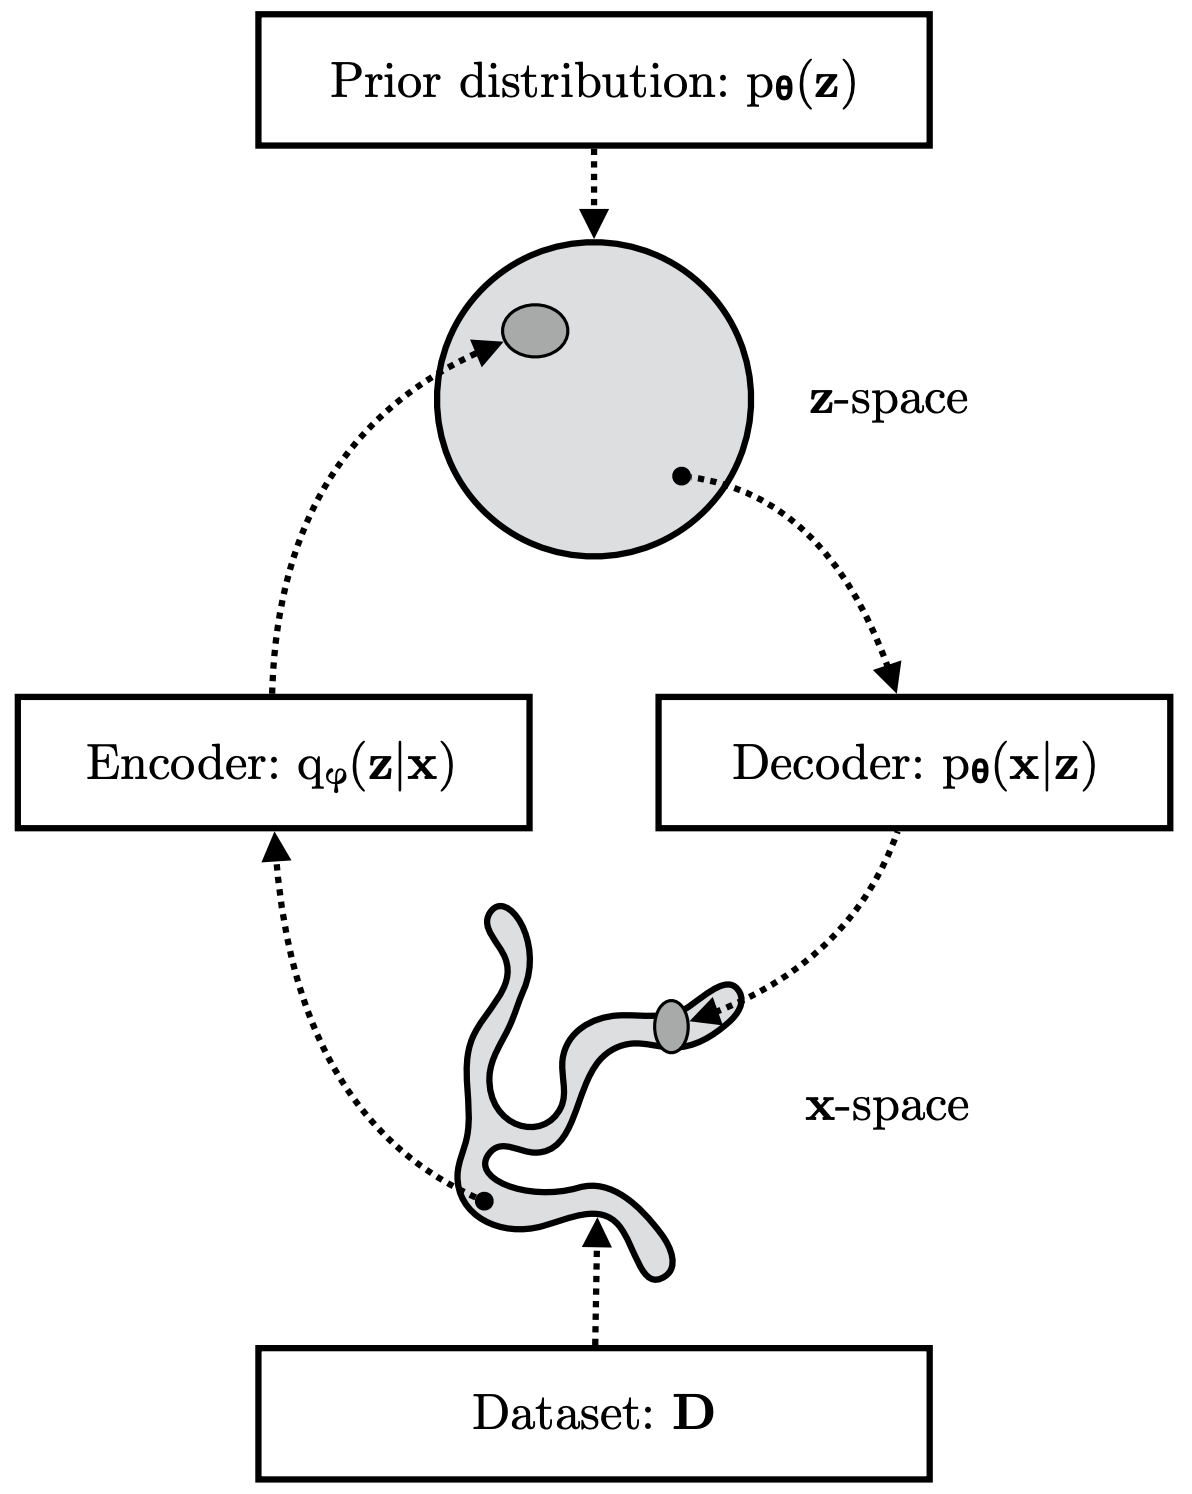
\includegraphics[width=\linewidth]{figs/vae_scheme}
		\end{figure}
	\end{minipage}
	
	\myfootnotewithlink{https://arxiv.org/abs/1906.02691}{Kingma D. P., Welling M. An introduction to variational autoencoders, 2019}
\end{frame}
%=======
\begin{frame}{Variational Autoencoder}
	\begin{figure}[h]
		\centering
		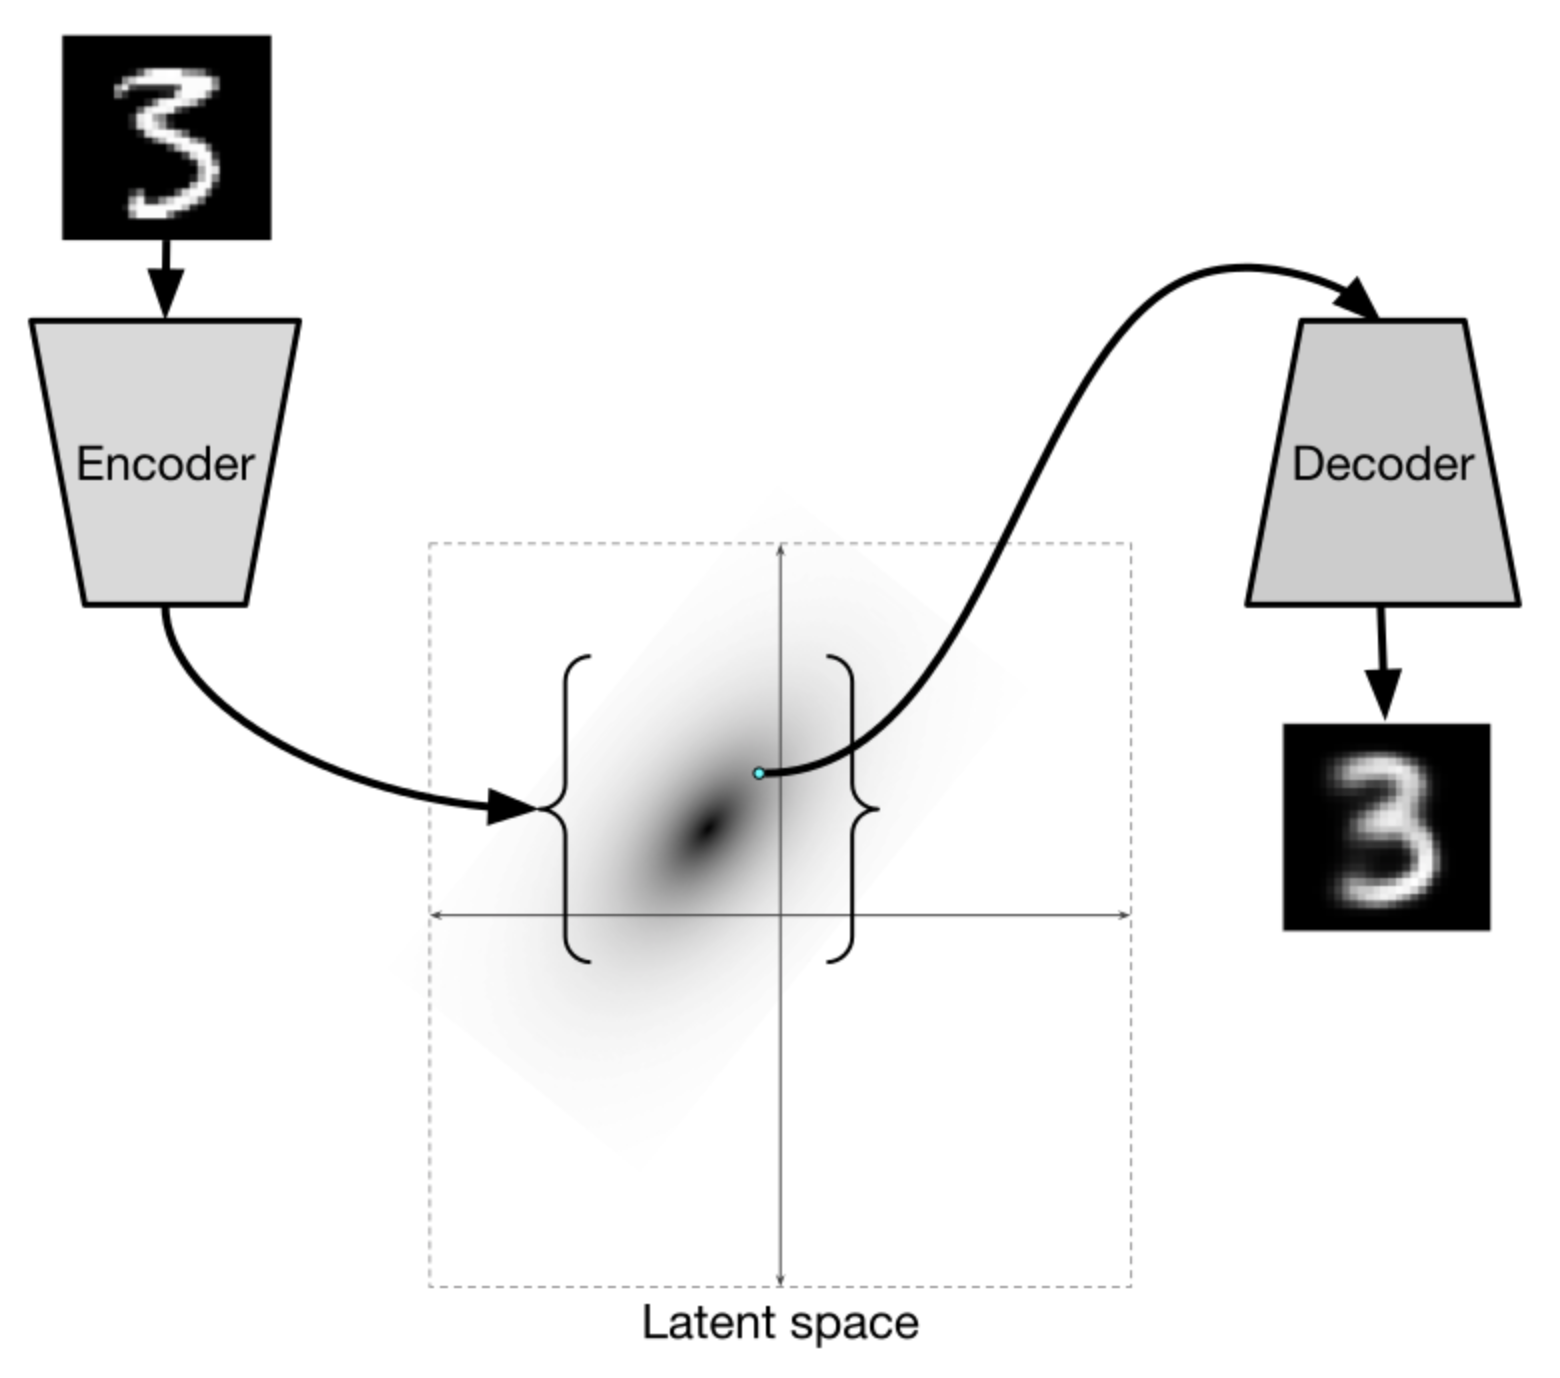
\includegraphics[width=.7\linewidth]{figs/VAE.png}
	\end{figure}
	\myfootnotewithlink{http://ijdykeman.github.io/ml/2016/12/21/cvae.html}{image credit: http://ijdykeman.github.io/ml/2016/12/21/cvae.html}
\end{frame}
%=======
\begin{frame}{Variational autoencoder (VAE)}
	\begin{itemize}
		\item Encoder $q(\bz | \bx, \bphi) = \text{NN}_e(\bx, \bphi)$ outputs $\bmu_{\bphi}(\bx)$ and $\bsigma_{\bphi}(\bx)$.
		\item Decoder $p(\bx | \bz, \btheta) = \text{NN}_d(\bz, \btheta)$ outputs parameters of the sample distribution.
	\end{itemize}
	\begin{figure}[h]
		\centering
		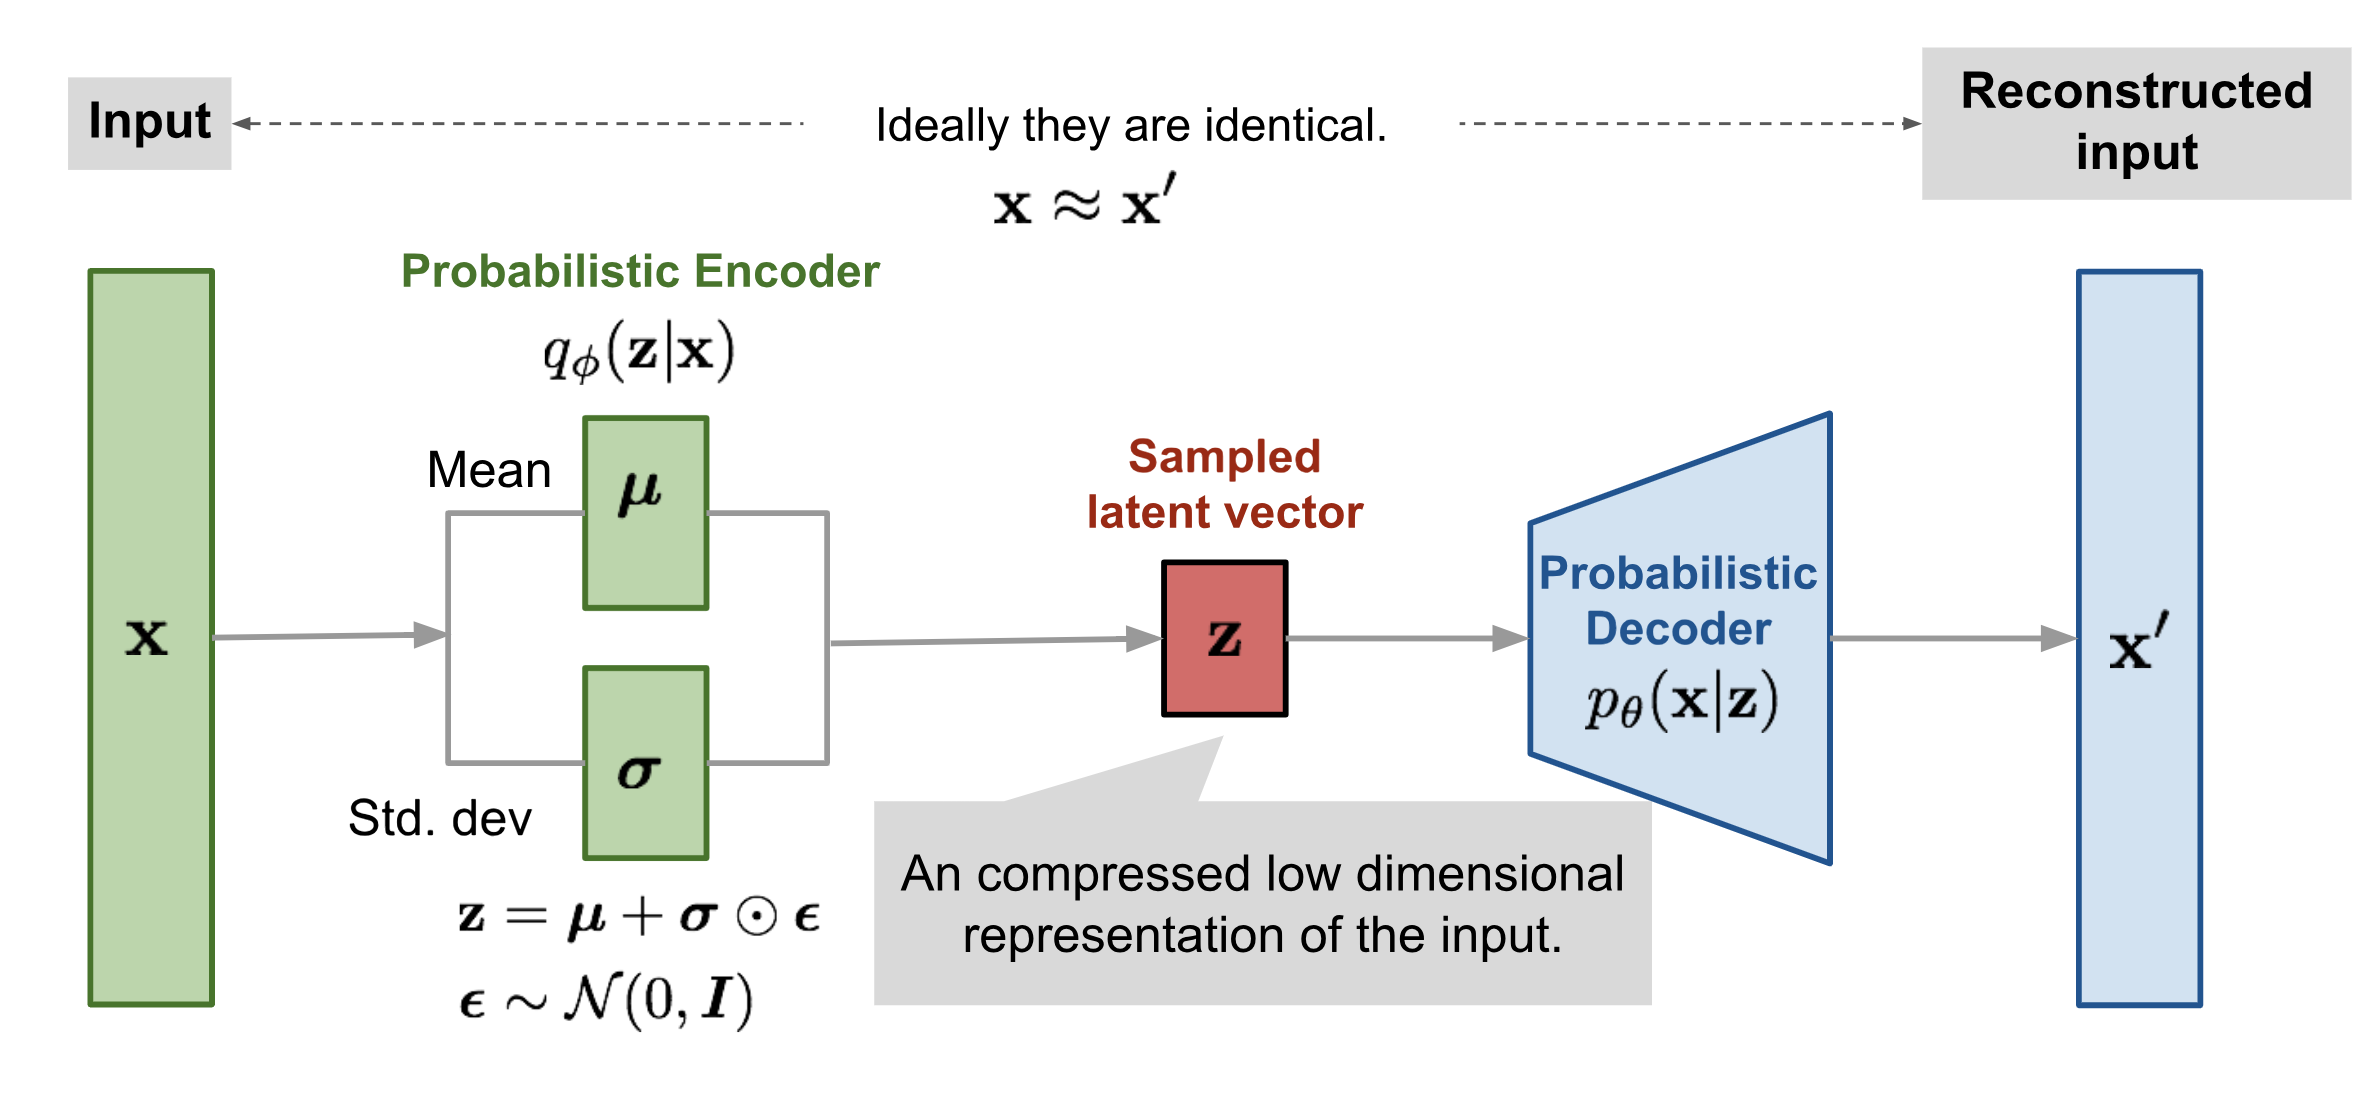
\includegraphics[width=\linewidth]{figs/vae-gaussian.png}
	\end{figure}
	
	\myfootnotewithlink{https://lilianweng.github.io/lil-log/2018/08/12/from-autoencoder-to-beta-vae.html}{image credit: https://lilianweng.github.io/lil-log/2018/08/12/from-autoencoder-to-beta-vae.html}
\end{frame}
%=======
\begin{frame}{Variational Autoencoder}
	Generated images for latent objects $\bz$ sampled from prior $\mathcal{N}(0, \mathbf{I})$
	\begin{figure}[h]
		\centering
		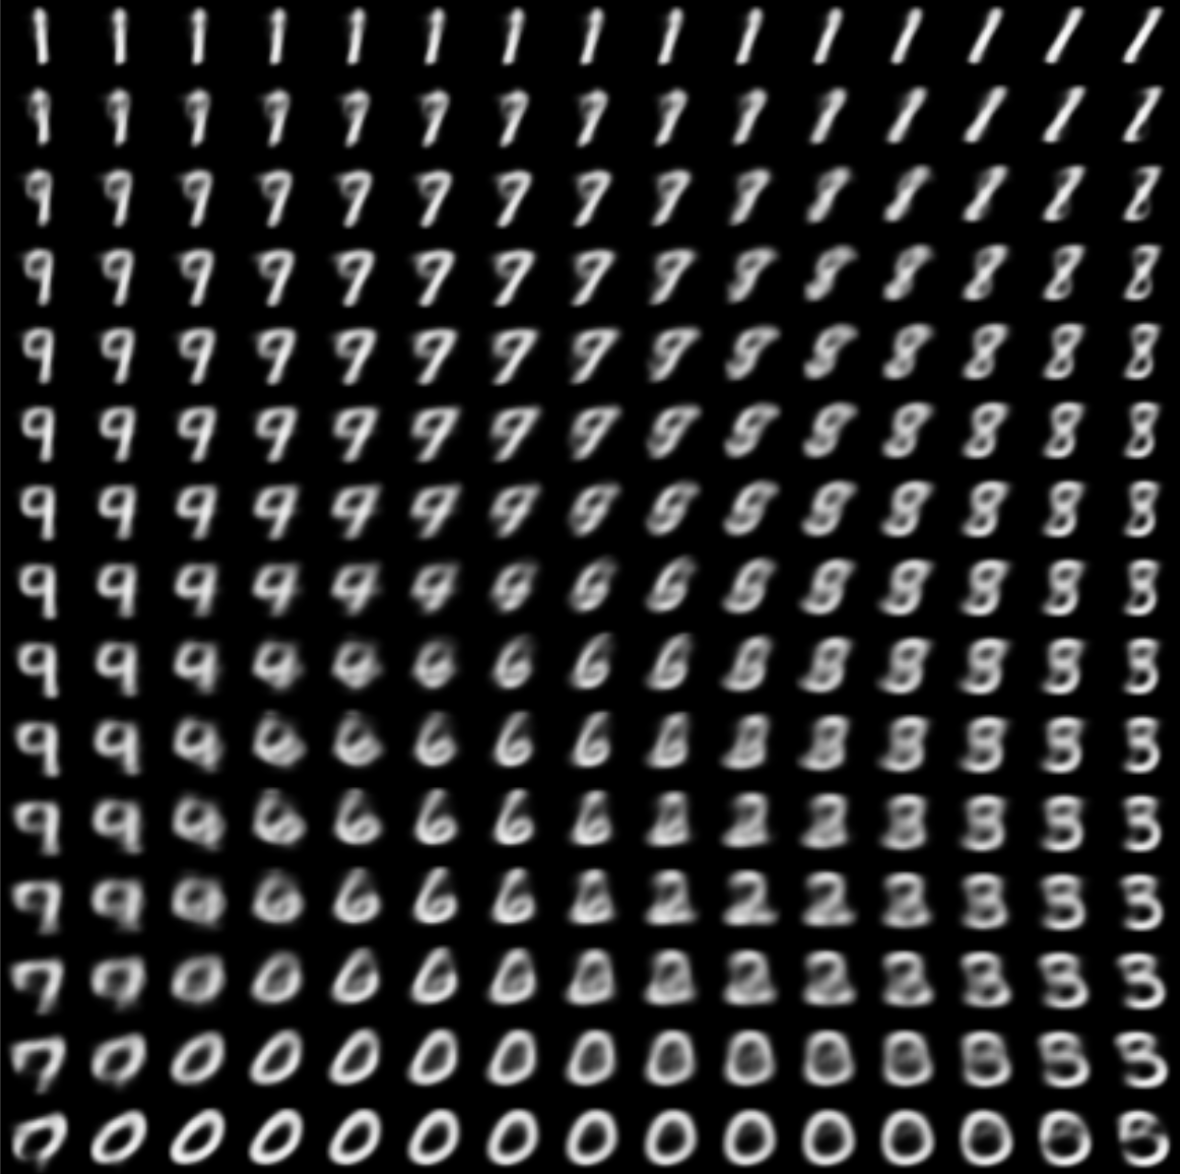
\includegraphics[width=.5\linewidth]{figs/vae_0.png}
	\end{figure}
	\myfootnotewithlink{https://habr.com/ru/post/331664}{image credit: https://habr.com/ru/post/331664}
\end{frame}
%=======
\begin{frame}{Bayesian framework}
	\begin{block}{Posterior distribution}
		\vspace{-0.2cm}
		\[
			p(\btheta | \bX) = \frac{p(\bX | \btheta) p(\btheta)}{p(\bX)} = \frac{p(\bX | \btheta) p(\btheta)}{\int p(\bX | \btheta) p(\btheta) d \btheta} 
		\]
		\vspace{-0.2cm}
	\end{block}
	\begin{block}{Bayesian inference}
		\vspace{-0.3cm}
		\[
			p(\bx | \bX) = \int p(\bx | \btheta) p(\btheta | \bX) d \btheta
		\]
	\end{block}
    \begin{block}{Maximum a posteriori (MAP) estimation}
	    \vspace{-0.3cm}
	    \[
	        \btheta^* = \argmax_{\btheta} \log p(\btheta | \bX) = \argmax_{\btheta} \bigl(\log p(\bX | \btheta) + \log p(\btheta) \bigr)
	    \]
        \vspace{-0.3cm}
    \end{block}
	\begin{block}{MAP inference}
		\vspace{-0.4cm}
		\[
			p(\bx | \bX) = \int p(\bx| \btheta) p(\btheta | \bX ) d \btheta =  \int p(\bx| \btheta) \delta (\btheta - \btheta^* ) d \btheta \approx p(\bx | \btheta^*).
		\]
	\end{block}
\end{frame}
%=======
\begin{frame}{VAE as Bayesian model}
	\begin{block}{Posterior distribution}
		\vspace{-0.2cm}
		\[
			p(\btheta | \bX) = \frac{p(\bX | \btheta) p(\btheta)}{p(\bX)}
		\]
		\vspace{-0.5cm}
	\end{block}
	\begin{block}{ELBO}
		\vspace{-0.5cm}
		\begin{align*}
			 \log p(\btheta | \bX) &= \log p(\bX | \btheta) + \log p(\btheta) - \log p(\bX) \\
			 &= \cL(q, \btheta) + KL(q || p) + \log p(\btheta) - \log p(\bX) \\
			 &\geq \left[ \cL(q, \btheta) + \log p(\btheta) \right] - \log p(\bX) .
		\end{align*}
		\vspace{-0.7cm}
	\end{block}
	\begin{block}{EM-algorithm}
		\begin{itemize}
			\item E-step
				\vspace{-0.2cm}
				\[
					q(\bz) = \argmax_q \mathcal{L} (q, \btheta^*) = \argmin_q KL(q || p) =
				 p(\bz| \bx, \btheta^*);
				\]
				\vspace{-0.5cm}
			\item M-step
				\[
					\btheta^* = \argmax_{\btheta} \left[ \mathcal{L} (q, \btheta) + \log p(\btheta) \right].
				\]
		\end{itemize}
	\end{block}
\end{frame}
%=======
\begin{frame}{VAE limitations}
	\begin{itemize}
		\item Poor variational posterior distribution (inference model encoder)
		\[
		q(\bz | \bx, \bphi) = \mathcal{N}(\bz| \bmu_{\bphi}(\bx), \bsigma^2_{\bphi}(\bx)).
		\]
		\item Poor prior distribution
		\[
		p(\bz) = \mathcal{N}(0, \mathbf{I}).
		\]
		\item Poor probabilistic model (generative model, decoder)
		\[
		p(\bx | \bz, \btheta) = \mathcal{N}(\bx| \bmu_{\btheta}(\bz), \bsigma^2_{\btheta}(\bz)).
		\]
		\item Loose lower bound
		\[
		\log p(\bx | \btheta) - \mathcal{L}(q, \btheta) = (?).
		\]
	\end{itemize}
\end{frame}
%=======
\begin{frame}{Summary}
	\begin{itemize}
		\item LVM maximizes variational evidence lower bound to find MLE of model parameters.
		\vfill
		\item ELBO maximization is performed by the general variational EM algorithm.
		\vfill
		\item Amortized inference allows to efficiently compute stochastic gradients for ELBO and to use deep neural networks for $q(\bz | \bx, \bphi)$ and $p(\bx | \bz, \btheta)$.
		\vfill
		\item ELBO gradients are computed using Monte-Carlo estimation.
		\vfill
		\item The reparametrization trick allows to get unbiased gradients w.r.t to a variational posterior distribution.
		\vfill
		\item The VAE model is an LVM with an encoder network for $q(\bz | \bx, \bphi)$ and a decoder network for $p(\bx | \bz, \btheta)$.
		\vfill
		\item VAE is not a "true" bayesian model since parameters $\btheta$ do not have a prior distribution.
		\vfill
		\item Standart VAE has several limitations that we will address later in the course.
	\end{itemize}
\end{frame}
%=======
\end{document} 